This section presents the results from the experiments we performed. We did not perform the analysis for the different types of graphs and also did not include bucket elimination. This is due to the fact that the implementation for these are not stable. So we first start with the random graph type in Subsection~\ref{subsec:ResultsRandom}. Then we will give a brief explanation why the implementation is unstable for the otehr types of graphs in Subsection~\ref{subsec:ResultsOtherTypes} and for bucket elimination in Subsection~\ref{subsec:ResultsBucket}. 

\subsection{Random Graphs} \label{subsec:ResultsRandom}
This subsection presents the results for the random graphs. In each graph the dots represent the measurement and the dotted line the trend line. The $y$-axis always represents the time in nanoseconds and the $x$-axis represents the variable quantity. So in case of the fixed order this is the density and in case of the fixed density this is the order. In each graph the different approaches are labelled with a colour. Blue stands for the naive approach, orange for straightforward, grey for early projection and yellow for the reordering approach.

  Figure~\ref{fig:ResultsRandomOrder} shows the results for the experiment in which the order was fixed. The fixed value for the order is 20. The density ranges from 0.5 to 12.5 with steps of 0.5. Figure~\ref{fig:ResultsRandomDensity2} presents the results for the experiment in which the density was fixed at 0.3. The order ranges from 10 till 27 with steps of 1. Figure~\ref{fig:ResultsRandomDensity3} present the result when the density is fixed to 0.6. The order, again, ranges from 10 till 27 with steps of 1. 
  
 The ranges presented in the graphs are maximal for our configuration and implementation. When we try to exceed beyond this point the RAM start slowly filling up. When we look at what takes up this increase of RAM it is PostgresSQL and not Java. Therefore we know that it is not the query generator but the query executor. In Section~\ref{sec:Discussion} we will come back to why we think this happens. 

\begin{figure}[h]
\center
	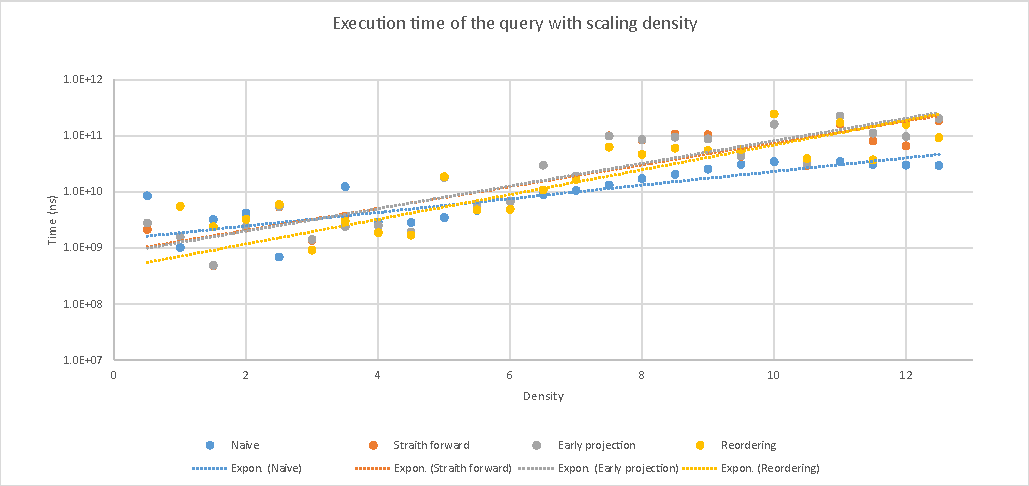
\includegraphics[width=0.9\textwidth]{figures/results_random_order}%[1cm]
	\caption{Graph presenting the results for the random graph type with a fixed order (20)}
	\label{fig:ResultsRandomOrder}
\end{figure}
\begin{figure}[h]
\center
	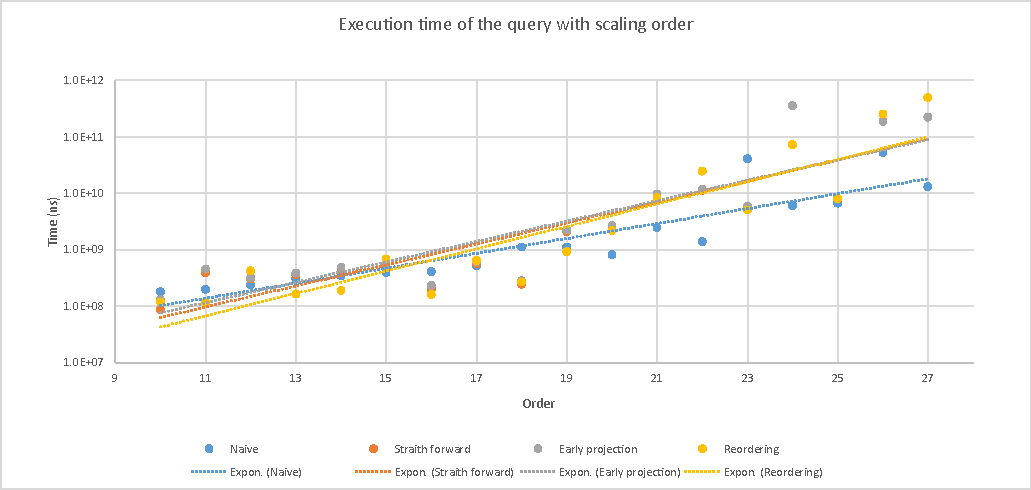
\includegraphics[width=0.9\textwidth]{figures/results_random_density2}%[1cm]
	\caption{Graph presenting the results for the random graph type with a fixed density (0.3)}
	\label{fig:ResultsRandomDensity2}
\end{figure}
\begin{figure}[h]
\center
	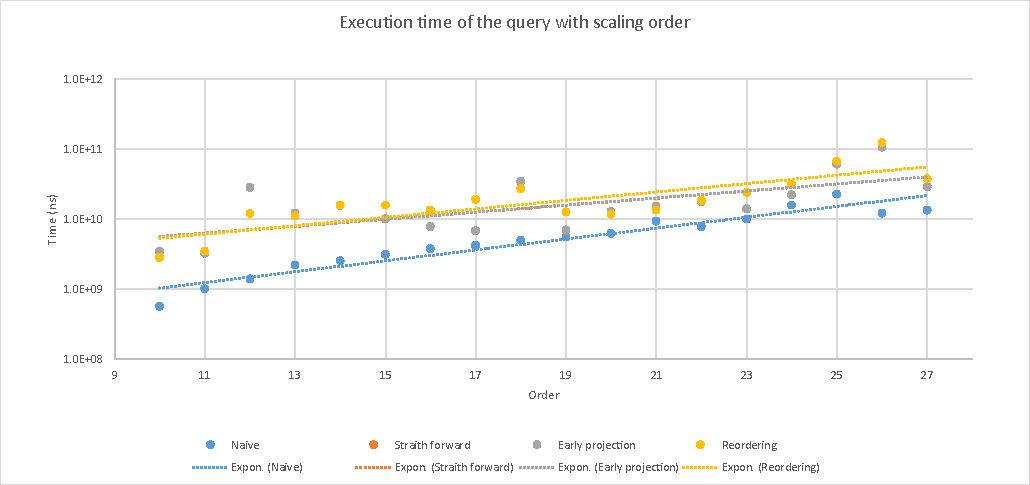
\includegraphics[width=0.9\textwidth]{figures/results_random_density3}%[1cm]
	\caption{Graph presenting the results for the random graph type with a fixed density (0.6)}
	\label{fig:ResultsRandomDensity3}
\end{figure}

\subsection{Other Types of Graphs} \label{subsec:ResultsOtherTypes}
As already mentioned before we were not able to run the experiments for the other types of graphs. This is due to the instability of the current state of the implementation. More specifically, the query generator has some issues. The graphs that are generated are generated correctly, but the query generators uses some attributes of the graph data structure and these appear not to be working properly. 

\subsection{Bucket Elimination} \label{subsec:ResultsBucket}
Bucket elimination was also not possible to include in the experiments. We tried to focus on the bucket elimination approach as the authors of out paper \cite{paper} claim that it is better than all the other approaches used. Unfortunately we did not had enough time to fix all the bugs that popped up in the last two weeks. 